\documentclass[12pt]{article}

\usepackage{fullpage}
\usepackage{framed}
\usepackage{standalone}
\usepackage{amsmath}
\usepackage{tikz}

\begin{document}
\part*{Glossary}
\begin{table}[!htb]
\begin{tabular}{rl}
\noindent \textbf{Basic Stats} &  a set of statistics that display: average contribution, total number \\ 
& of contributors and total lines of code in the repository.\\

& \\

\noindent \textbf{Method}    & a group of commands grouped together to perform an operation \\
& (like a `function')\\

& \\                             

\noindent \textbf{Tool-Tip} & a small message which appears when a cursor is positioned over an image,\\
                             &  text or hyperlink.\\
                             & \hfill 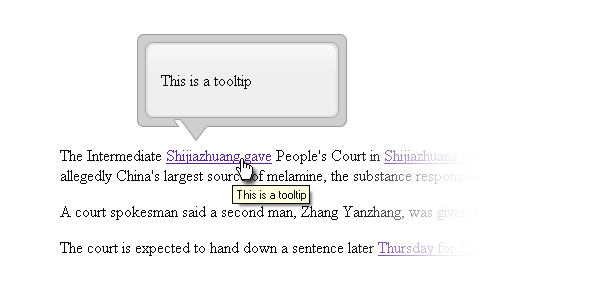
\includegraphics[scale=0.7]{tooltip}\\
                             & \\
                             & \\
                             & \\
                             & \\
                             & \\
                             & \\
\end{tabular}
\end{table}
\end{document}